% ============================================================================
% UNIFY -- Diagram 6 (Haaniah)
% State machines: event processing, source freshness, finding lifecycle
% Traces to proposal v2 sec. 8.4 (reliability), 11.7 (verdict semantics),
% FR-16 (SOURCE_STALE) and FR-18 (finding lifecycle actions)
% Build: pdflatex 06_state_machines.tex
% ============================================================================
\documentclass[border=12pt]{standalone}
% =============================================================================
% UNIFY -- shared TikZ style used by Haaniah's self-contained diagrams
%          (05_ingestion_sequence.tex, 06_state_machines.tex, 11_deployment.tex)
%
% Those three files each start with \documentclass{standalone} + % =============================================================================
% UNIFY -- shared TikZ style used by Haaniah's self-contained diagrams
%          (05_ingestion_sequence.tex, 06_state_machines.tex, 11_deployment.tex)
%
% Those three files each start with \documentclass{standalone} + % =============================================================================
% UNIFY -- shared TikZ style used by Haaniah's self-contained diagrams
%          (05_ingestion_sequence.tex, 06_state_machines.tex, 11_deployment.tex)
%
% Those three files each start with \documentclass{standalone} + \input{unifystyle}
% and are compiled on their own ("pdflatex <file>.tex"), unlike Mishal's and
% Abdullah's sources, which are fragments wrapped by build.sh.
%
% The original unifystyle.tex was never committed. This file was reconstructed
% so the folder is self-contained again: the palette below was sampled directly
% from the committed renders (rendered/*.png, 200 dpi), and the geometry was
% matched against them. A rebuild should reproduce the committed PDFs closely;
% if you edit a style here, re-render all three and eyeball the diff.
%
% Layout note: like unify-diagram-styles.tex, this is plain TikZ (no tikz-uml),
% so it compiles in any TeX Live.
% =============================================================================
% Times, to match the report body and the fragment diagrams
\usepackage{mathptmx}
\usepackage[T1]{fontenc}
\usepackage{tikz}
\usepackage{pgffor} % \foreach (05_ingestion_sequence lifelines)
\usetikzlibrary{arrows.meta,positioning,calc,fit,backgrounds,
                shapes.geometric,shapes.multipart,decorations.pathreplacing}

% ---- palette: exact fills sampled from the committed renders ----------------
\definecolor{extgrey}{HTML}{EDEDED}    % vendor / superseded (neutral)
\definecolor{relblue}{HTML}{CFE2F3}    % pipeline steps, fresh path
\definecolor{graphgreen}{HTML}{D9EAD3} % evidence graph / applied
\definecolor{verorange}{HTML}{FCE5CD}  % verification / findings / model
\definecolor{badred}{HTML}{F8D7DA}     % rejected / SOURCE_STALE
\definecolor{okgreen}{HTML}{DFF0D8}    % discarded / ignored / resolved
\definecolor{warnamber}{HTML}{FCE8C3}  % degraded / disputed
\definecolor{hynote}{HTML}{FFF9D6}     % side-note boxes

\tikzset{
  % ---- 05: sequence diagram --------------------------------------------------
  lane/.style={draw, fill=#1, rounded corners=2pt, inner sep=4pt,
               align=center, font=\bfseries\scriptsize},
  frame/.style={draw},                       % sdframe rectangles
  ftab/.style={draw, fill=white, font=\scriptsize, inner sep=1.5pt}, % alt A tab
  msg/.style={-{Stealth[length=2.5mm]}},     % call arrow
  ret/.style={-{Stealth[length=2.5mm]}, dashed}, % return arrow
  box/.style={draw, fill=#1, rounded corners=2pt, inner sep=4pt, align=center},
  % ---- 06: state machines ----------------------------------------------------
  st/.style={draw, fill=#1, rounded corners=2pt, inner sep=4pt,
             align=center, font=\scriptsize},
  dec/.style={diamond, aspect=1.75, draw, fill=white, font=\scriptsize,
              align=center, text width=1.5cm, inner sep=1pt},
  tr/.style={-{Stealth[length=2.2mm]}},       % state transition
  % ---- shared ----------------------------------------------------------------
  lbl/.style={font=\scriptsize, fill=white, inner sep=1pt},
  mlbl/.style={font=\scriptsize, align=center, inner sep=1pt}, % message label, sits above the arrow
  note/.style={draw, fill=hynote, font=\scriptsize, align=left,
               text width=#1, inner sep=4pt, rounded corners=2pt},
  note/.default=4.6cm,
}

% and are compiled on their own ("pdflatex <file>.tex"), unlike Mishal's and
% Abdullah's sources, which are fragments wrapped by build.sh.
%
% The original unifystyle.tex was never committed. This file was reconstructed
% so the folder is self-contained again: the palette below was sampled directly
% from the committed renders (rendered/*.png, 200 dpi), and the geometry was
% matched against them. A rebuild should reproduce the committed PDFs closely;
% if you edit a style here, re-render all three and eyeball the diff.
%
% Layout note: like unify-diagram-styles.tex, this is plain TikZ (no tikz-uml),
% so it compiles in any TeX Live.
% =============================================================================
% Times, to match the report body and the fragment diagrams
\usepackage{mathptmx}
\usepackage[T1]{fontenc}
\usepackage{tikz}
\usepackage{pgffor} % \foreach (05_ingestion_sequence lifelines)
\usetikzlibrary{arrows.meta,positioning,calc,fit,backgrounds,
                shapes.geometric,shapes.multipart,decorations.pathreplacing}

% ---- palette: exact fills sampled from the committed renders ----------------
\definecolor{extgrey}{HTML}{EDEDED}    % vendor / superseded (neutral)
\definecolor{relblue}{HTML}{CFE2F3}    % pipeline steps, fresh path
\definecolor{graphgreen}{HTML}{D9EAD3} % evidence graph / applied
\definecolor{verorange}{HTML}{FCE5CD}  % verification / findings / model
\definecolor{badred}{HTML}{F8D7DA}     % rejected / SOURCE_STALE
\definecolor{okgreen}{HTML}{DFF0D8}    % discarded / ignored / resolved
\definecolor{warnamber}{HTML}{FCE8C3}  % degraded / disputed
\definecolor{hynote}{HTML}{FFF9D6}     % side-note boxes

\tikzset{
  % ---- 05: sequence diagram --------------------------------------------------
  lane/.style={draw, fill=#1, rounded corners=2pt, inner sep=4pt,
               align=center, font=\bfseries\scriptsize},
  frame/.style={draw},                       % sdframe rectangles
  ftab/.style={draw, fill=white, font=\scriptsize, inner sep=1.5pt}, % alt A tab
  msg/.style={-{Stealth[length=2.5mm]}},     % call arrow
  ret/.style={-{Stealth[length=2.5mm]}, dashed}, % return arrow
  box/.style={draw, fill=#1, rounded corners=2pt, inner sep=4pt, align=center},
  % ---- 06: state machines ----------------------------------------------------
  st/.style={draw, fill=#1, rounded corners=2pt, inner sep=4pt,
             align=center, font=\scriptsize},
  dec/.style={diamond, aspect=1.75, draw, fill=white, font=\scriptsize,
              align=center, text width=1.5cm, inner sep=1pt},
  tr/.style={-{Stealth[length=2.2mm]}},       % state transition
  % ---- shared ----------------------------------------------------------------
  lbl/.style={font=\scriptsize, fill=white, inner sep=1pt},
  mlbl/.style={font=\scriptsize, align=center, inner sep=1pt}, % message label, sits above the arrow
  note/.style={draw, fill=hynote, font=\scriptsize, align=left,
               text width=#1, inner sep=4pt, rounded corners=2pt},
  note/.default=4.6cm,
}

% and are compiled on their own ("pdflatex <file>.tex"), unlike Mishal's and
% Abdullah's sources, which are fragments wrapped by build.sh.
%
% The original unifystyle.tex was never committed. This file was reconstructed
% so the folder is self-contained again: the palette below was sampled directly
% from the committed renders (rendered/*.png, 200 dpi), and the geometry was
% matched against them. A rebuild should reproduce the committed PDFs closely;
% if you edit a style here, re-render all three and eyeball the diff.
%
% Layout note: like unify-diagram-styles.tex, this is plain TikZ (no tikz-uml),
% so it compiles in any TeX Live.
% =============================================================================
% Times, to match the report body and the fragment diagrams
\usepackage{mathptmx}
\usepackage[T1]{fontenc}
\usepackage{tikz}
\usepackage{pgffor} % \foreach (05_ingestion_sequence lifelines)
\usetikzlibrary{arrows.meta,positioning,calc,fit,backgrounds,
                shapes.geometric,shapes.multipart,decorations.pathreplacing}

% ---- palette: exact fills sampled from the committed renders ----------------
\definecolor{extgrey}{HTML}{EDEDED}    % vendor / superseded (neutral)
\definecolor{relblue}{HTML}{CFE2F3}    % pipeline steps, fresh path
\definecolor{graphgreen}{HTML}{D9EAD3} % evidence graph / applied
\definecolor{verorange}{HTML}{FCE5CD}  % verification / findings / model
\definecolor{badred}{HTML}{F8D7DA}     % rejected / SOURCE_STALE
\definecolor{okgreen}{HTML}{DFF0D8}    % discarded / ignored / resolved
\definecolor{warnamber}{HTML}{FCE8C3}  % degraded / disputed
\definecolor{hynote}{HTML}{FFF9D6}     % side-note boxes

\tikzset{
  % ---- 05: sequence diagram --------------------------------------------------
  lane/.style={draw, fill=#1, rounded corners=2pt, inner sep=4pt,
               align=center, font=\bfseries\scriptsize},
  frame/.style={draw},                       % sdframe rectangles
  ftab/.style={draw, fill=white, font=\scriptsize, inner sep=1.5pt}, % alt A tab
  msg/.style={-{Stealth[length=2.5mm]}},     % call arrow
  ret/.style={-{Stealth[length=2.5mm]}, dashed}, % return arrow
  box/.style={draw, fill=#1, rounded corners=2pt, inner sep=4pt, align=center},
  % ---- 06: state machines ----------------------------------------------------
  st/.style={draw, fill=#1, rounded corners=2pt, inner sep=4pt,
             align=center, font=\scriptsize},
  dec/.style={diamond, aspect=1.75, draw, fill=white, font=\scriptsize,
              align=center, text width=1.5cm, inner sep=1pt},
  tr/.style={-{Stealth[length=2.2mm]}},       % state transition
  % ---- shared ----------------------------------------------------------------
  lbl/.style={font=\scriptsize, fill=white, inner sep=1pt},
  mlbl/.style={font=\scriptsize, align=center, inner sep=1pt}, % message label, sits above the arrow
  note/.style={draw, fill=hynote, font=\scriptsize, align=left,
               text width=#1, inner sep=4pt, rounded corners=2pt},
  note/.default=4.6cm,
}


\begin{document}
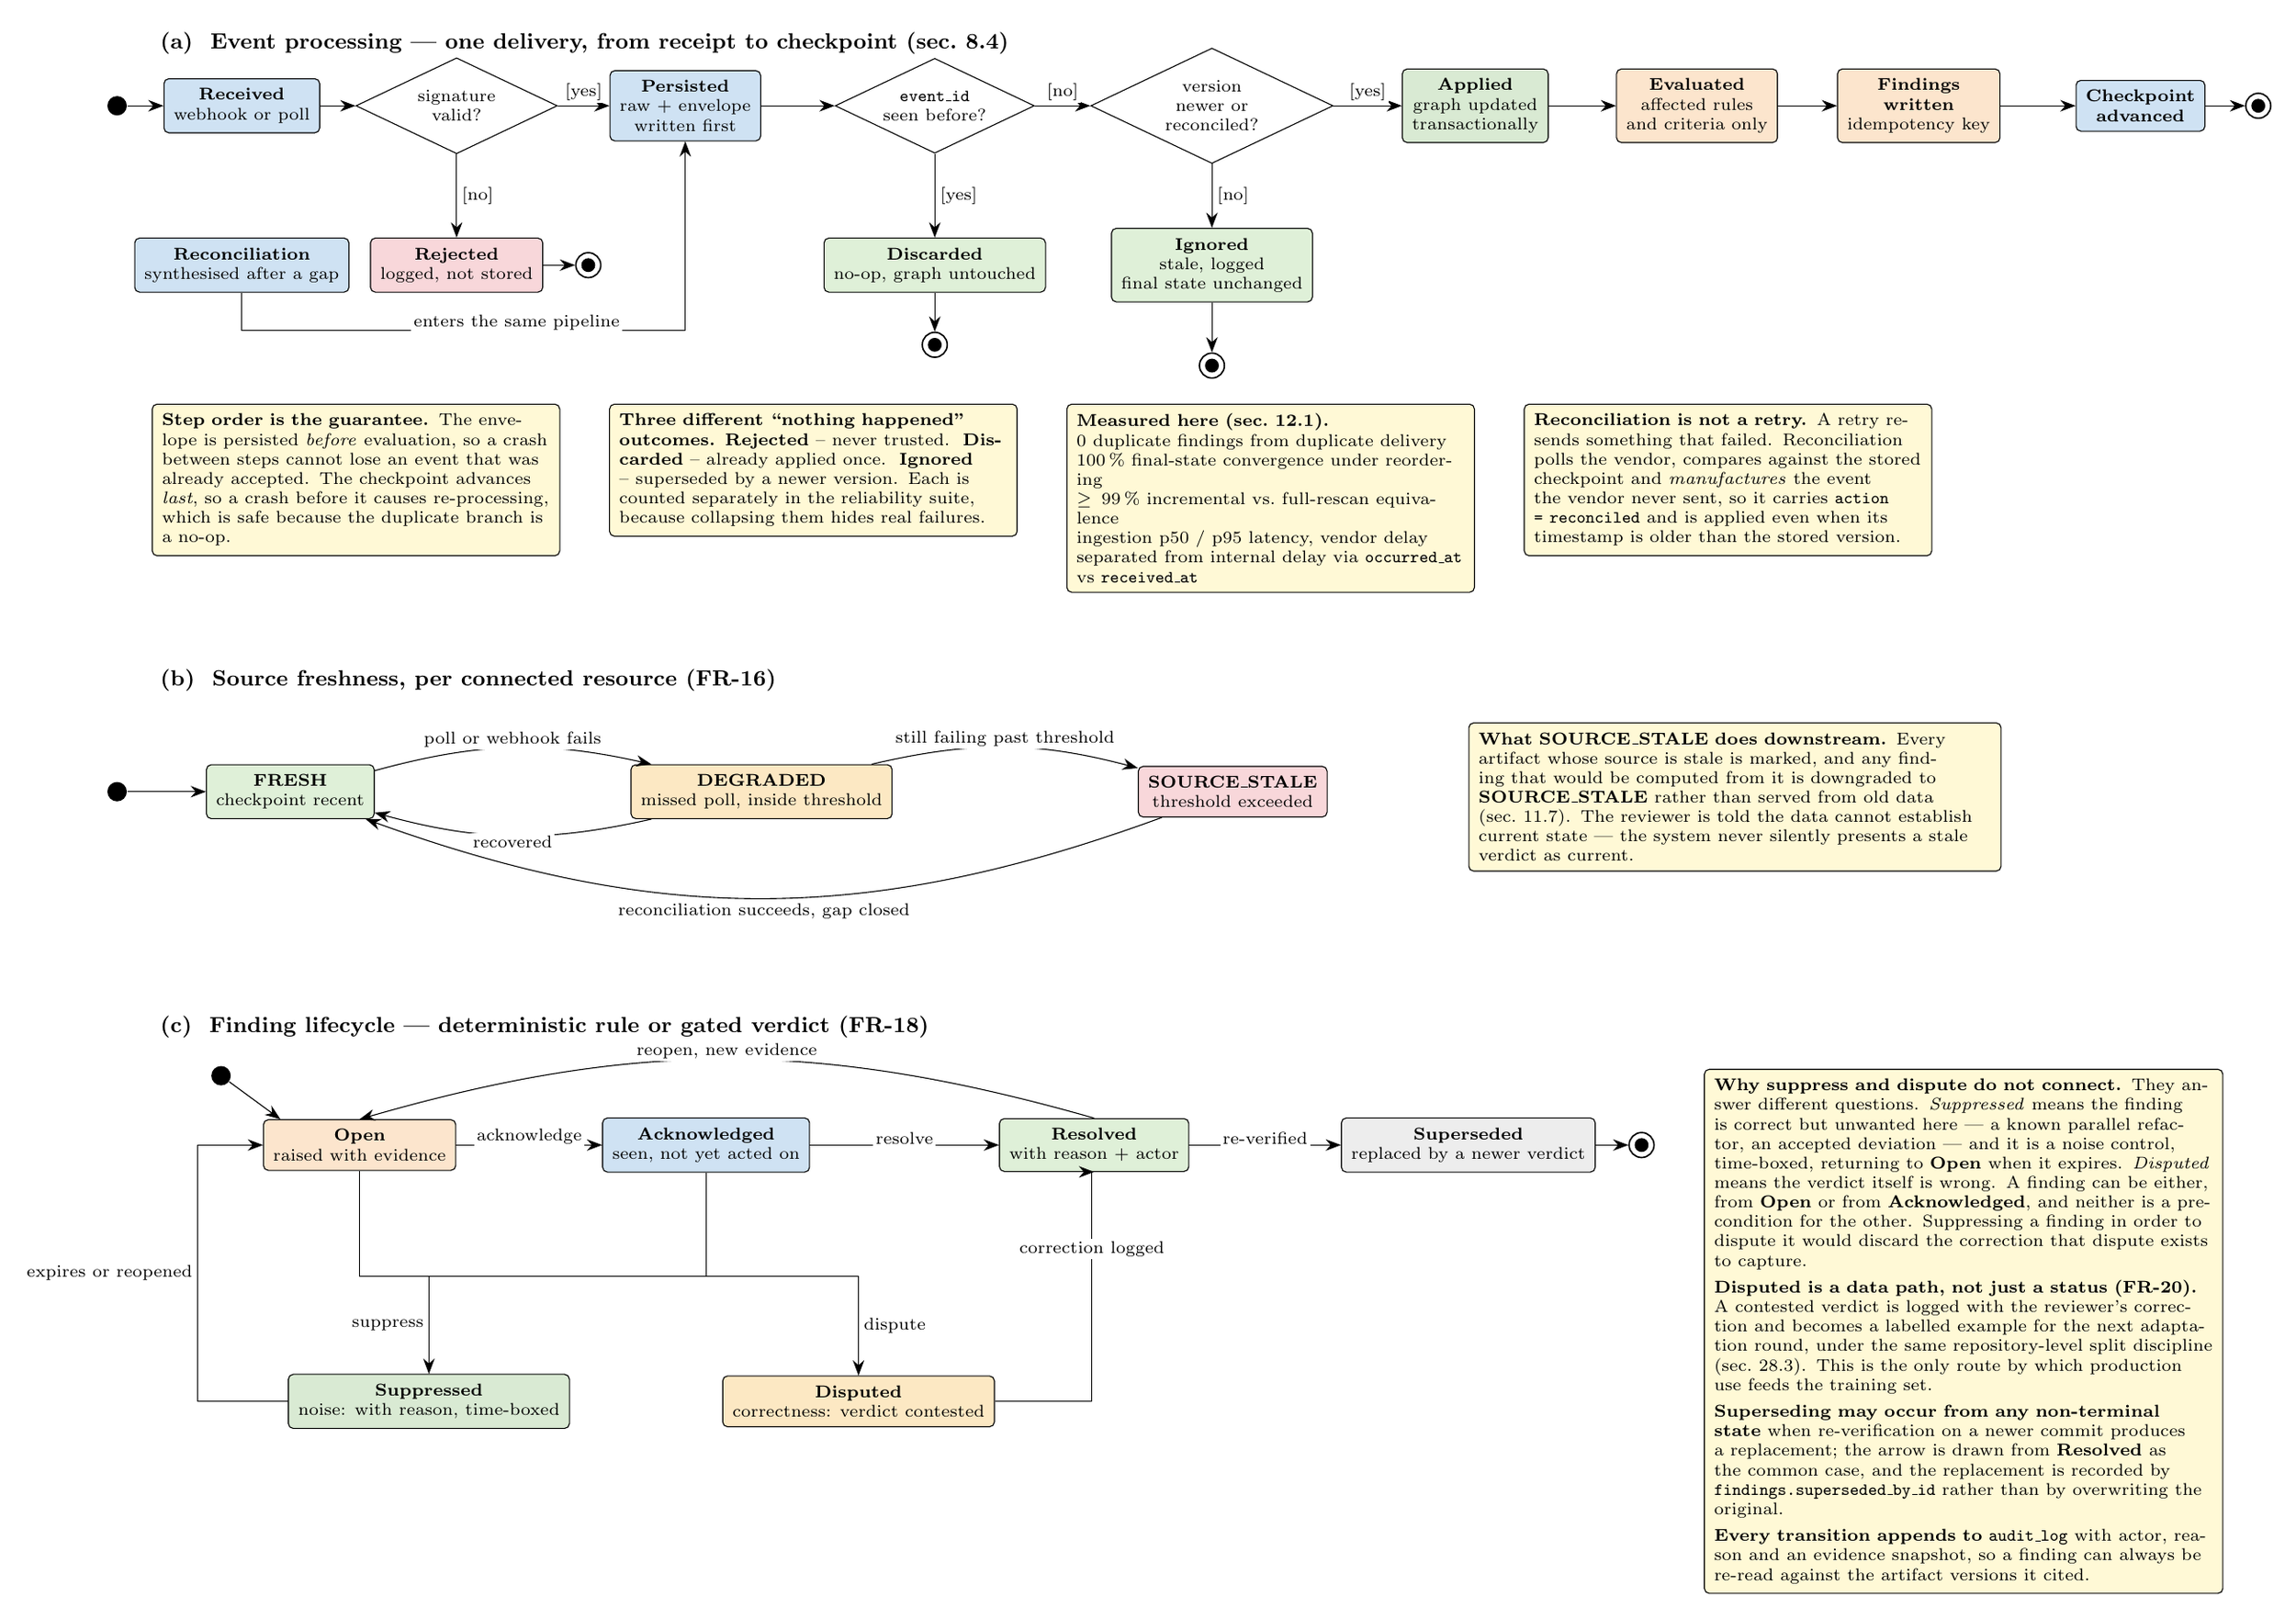
\begin{tikzpicture}[x=1cm,y=1cm,node distance=0pt]
\tikzset{init/.style={circle, fill=black, minimum size=0.28cm, inner sep=0pt},
         final/.style={circle, draw, line width=0.6pt, minimum size=0.36cm,
                       inner sep=0pt, path picture={\fill[black]
                       (path picture bounding box.center) circle (0.1cm);}},
         dec/.append style={text width=1.75cm, aspect=2.1}}

% ===================== PANEL A : event processing =======================
\node[font=\bfseries\small,anchor=west] at (-0.4,0.9)
  {(a)\ \ Event processing --- one delivery, from receipt to checkpoint (sec.~8.4)};

\node[st=relblue]   (recv)  at ( 0.9, 0)   {\textbf{Received}\\\scriptsize webhook or poll};
\node[dec]          (auth)  at ( 4.0, 0)   {signature\\valid?};
\node[st=relblue]   (pers)  at ( 7.3, 0)   {\textbf{Persisted}\\\scriptsize raw + envelope\\\scriptsize written first};
\node[dec]          (dup)   at (10.9, 0)   {\texttt{event\_id}\\seen before?};
\node[dec]          (ver)   at (14.9, 0)   {version newer or\\reconciled?};
\node[st=graphgreen](appl)  at (18.7, 0)   {\textbf{Applied}\\\scriptsize graph updated\\\scriptsize transactionally};
\node[st=verorange] (eval)  at (21.9, 0)   {\textbf{Evaluated}\\\scriptsize affected rules\\\scriptsize and criteria only};
\node[st=verorange] (writ)  at (25.1, 0)   {\textbf{Findings}\\\textbf{written}\\\scriptsize idempotency key};
\node[st=relblue]   (ckpt)  at (28.3, 0)   {\textbf{Checkpoint}\\\textbf{advanced}};

\node[st=badred]    (rej)   at ( 4.0,-2.3) {\textbf{Rejected}\\\scriptsize logged, not stored};
\node[st=okgreen]   (noop)  at (10.9,-2.3) {\textbf{Discarded}\\\scriptsize no-op, graph untouched};
\node[st=okgreen]   (ign)   at (14.9,-2.3) {\textbf{Ignored}\\\scriptsize stale, logged\\\scriptsize final state unchanged};

\draw[tr] (recv) -- (auth);
\draw[tr] (auth) -- node[lbl,above=1pt]{[yes]} (pers);
\draw[tr] (auth) -- node[lbl,right=1pt]{[no]} (rej);
\draw[tr] (pers) -- (dup);
\draw[tr] (dup)  -- node[lbl,right=1pt]{[yes]} (noop);
\draw[tr] (dup)  -- node[lbl,above=1pt]{[no]} (ver);
\draw[tr] (ver)  -- node[lbl,right=1pt]{[no]} (ign);
\draw[tr] (ver)  -- node[lbl,above=1pt]{[yes]} (appl);
\draw[tr] (appl) -- (eval);
\draw[tr] (eval) -- (writ);
\draw[tr] (writ) -- (ckpt);
% initial and final pseudostates
\node[init] (a0) at (-0.9,0) {};
\draw[tr] (a0) -- (recv);
\node[final] (af) at (30.0,0) {};
\draw[tr] (ckpt) -- (af);
\node[final] (rejf) at (5.9,-2.3) {};
\draw[tr] (rej) -- (rejf);
\node[final] (noopf) at (10.9,-3.45) {};
\draw[tr] (noop) -- (noopf);
\node[final] (ignf) at (14.9,-3.75) {};
\draw[tr] (ign) -- (ignf);

% reconciliation re-entry
\node[st=relblue] (rec) at (0.9,-2.3) {\textbf{Reconciliation}\\\scriptsize synthesised after a gap};
\draw[tr] (rec.south) -- ++(0,-0.55) -- node[lbl,above=-1pt,pos=.62]{enters the same pipeline} ++(6.4,0) -| (pers.south);

\node[note=5.6cm,anchor=north west] at (-0.4,-4.3)
  {\textbf{Step order is the guarantee.}
   The envelope is persisted \emph{before} evaluation, so a crash between
   steps cannot lose an event that was already accepted. The checkpoint
   advances \emph{last}, so a crash before it causes re-processing, which is
   safe because the duplicate branch is a no-op.};

\node[note=5.6cm,anchor=north west] at (6.2,-4.3)
  {\textbf{Three different \lq\lq{}nothing happened\rq\rq{} outcomes.}
   \textbf{Rejected} -- never trusted.\ \ \textbf{Discarded} -- already
   applied once.\ \ \textbf{Ignored} -- superseded by a newer version.
   Each is counted separately in the reliability suite, because collapsing
   them hides real failures.};

\node[note=5.6cm,anchor=north west] at (12.8,-4.3)
  {\textbf{Measured here (sec.~12.1).}\\
   0 duplicate findings from duplicate delivery\\
   100\,\% final-state convergence under reordering\\
   $\geq 99\,\%$ incremental vs.\ full-rescan equivalence\\
   ingestion p50 / p95 latency, vendor delay separated
   from internal delay via \texttt{occurred\_at} vs \texttt{received\_at}};

\node[note=5.6cm,anchor=north west] at (19.4,-4.3)
  {\textbf{Reconciliation is not a retry.}
   A retry resends something that failed. Reconciliation polls the vendor,
   compares against the stored checkpoint and \emph{manufactures} the event
   the vendor never sent, so it carries
   \texttt{action = reconciled} and is applied even when its timestamp is
   older than the stored version.};

\begin{scope}[yshift=-1.0cm]
% ===================== PANEL B : source freshness =======================
\node[font=\bfseries\small,anchor=west] at (-0.4,-7.3)
  {(b)\ \ Source freshness, per connected resource (FR-16)};

\node[st=okgreen]  (fresh) at ( 1.6,-8.9) {\textbf{FRESH}\\\scriptsize checkpoint recent};
\node[st=warnamber](degr)  at ( 8.4,-8.9) {\textbf{DEGRADED}\\\scriptsize missed poll, inside threshold};
\node[st=badred]   (stale) at (15.2,-8.9) {\textbf{SOURCE\_STALE}\\\scriptsize threshold exceeded};

\node[init] (b0) at (-0.9,-8.9) {};
\draw[tr] (b0) -- (fresh);
\draw[tr] (fresh) to[bend left=14] node[lbl,above=-1pt]{poll or webhook fails} (degr);
\draw[tr] (degr)  to[bend left=14] node[lbl,below=-1pt]{recovered} (fresh);
\draw[tr] (degr)  to[bend left=14] node[lbl,above=-1pt]{still failing past threshold} (stale);
\draw[tr] (stale) to[bend left=20] node[lbl,below=1pt]{reconciliation succeeds, gap closed} (fresh);

\node[note=7.4cm,anchor=north west] at (18.6,-7.9)
  {\textbf{What SOURCE\_STALE does downstream.} Every artifact whose source
   is stale is marked, and any finding that would be computed from it is
   downgraded to \textbf{SOURCE\_STALE} rather than served from old data
   (sec.~11.7). The reviewer is told the data cannot establish current
   state --- the system never silently presents a stale verdict as current.};

\begin{scope}[yshift=-0.7cm]
% ===================== PANEL C : finding lifecycle ======================
\node[font=\bfseries\small,anchor=west] at (-0.4,-11.6)
  {(c)\ \ Finding lifecycle --- deterministic rule or gated verdict (FR-18)};

\node[st=verorange] (open)  at ( 2.6,-13.3) {\textbf{Open}\\\scriptsize raised with evidence};
\node[st=relblue]   (ack)   at ( 7.6,-13.3) {\textbf{Acknowledged}\\\scriptsize seen, not yet acted on};
\node[st=okgreen]   (res)   at (13.2,-13.3) {\textbf{Resolved}\\\scriptsize with reason + actor};
\node[st=extgrey]   (super) at (18.6,-13.3) {\textbf{Superseded}\\\scriptsize replaced by a newer verdict};
\node[st=graphgreen](sup)   at ( 3.6,-17.0) {\textbf{Suppressed}\\\scriptsize noise: with reason, time-boxed};
\node[st=warnamber] (disp)  at ( 9.8,-17.0) {\textbf{Disputed}\\\scriptsize correctness: verdict contested};

\node[init] (c0) at (0.6,-12.3) {};
\draw[tr] (c0) -- ([xshift=0.25cm]open.north west);
\node[final] (cf) at (21.1,-13.3) {};
\draw[tr] (super) -- (cf);
\draw[tr] (open) -- node[lbl,above=-1pt]{acknowledge} (ack);
\draw[tr] (ack)  -- node[lbl,above=-1pt]{resolve} (res);
\draw[tr] (res.north) to[bend right=16] node[lbl,above=-1pt]{reopen, new evidence} (open.north);
\draw[tr] (res) -- node[lbl,above=-1pt]{re-verified} (super);

% Suppress and dispute are independent responses, each available from Open and
% from Acknowledged. Shown as a shared bus so neither depends on the other.
\draw[tr,-] (open.south) -- (2.6,-15.2);
\draw[tr,-] (ack.south)  -- (7.6,-15.2);
\draw[tr,-] (2.6,-15.2)  -- (9.8,-15.2);
\draw[tr] (3.6,-15.2) -- node[lbl,left=1pt]{suppress} (sup.north);
\draw[tr] (9.8,-15.2) -- node[lbl,right=1pt]{dispute} (disp.north);

\draw[tr] (sup.west) -- ++(-1.3,0) |- node[lbl,left=1pt,pos=.25]{expires or reopened} (open.west);
\draw[tr] (disp.east) -- ++(1.4,0) |- node[lbl,below=-1pt,pos=.35]{correction logged} (res.south);

\node[note=7.2cm,anchor=north west] at (22.0,-12.2)
  {\textbf{Why suppress and dispute do not connect.}
   They answer different questions. \emph{Suppressed} means the finding is
   correct but unwanted here --- a known parallel refactor, an accepted
   deviation --- and it is a noise control, time-boxed, returning to
   \textbf{Open} when it expires. \emph{Disputed} means the verdict itself is
   wrong. A finding can be either, from \textbf{Open} or from
   \textbf{Acknowledged}, and neither is a precondition for the other.
   Suppressing a finding in order to dispute it would discard the correction
   that dispute exists to capture.\\[3pt]
   \textbf{Disputed is a data path, not just a status (FR-20).}
   A contested verdict is logged with the reviewer's correction and becomes a
   labelled example for the next adaptation round, under the same
   repository-level split discipline (sec.~28.3). This is the only route by
   which production use feeds the training set.\\[3pt]
   \textbf{Superseding may occur from any non-terminal state} when
   re-verification on a newer commit produces a replacement; the arrow is
   drawn from \textbf{Resolved} as the common case, and the replacement is
   recorded by \texttt{findings.superseded\_by\_id} rather than by
   overwriting the original.\\[3pt]
   \textbf{Every transition appends to \texttt{audit\_log}} with actor,
   reason and an evidence snapshot, so a finding can always be re-read
   against the artifact versions it cited.};

\end{scope}
\end{scope}
\end{tikzpicture}
\end{document}